\section{Introduction}

Large language models (LLMs) have inspired the development of a new generation of autonomous AI agents capable of planning, reasoning, and interacting with tools to solve complex problems that were traditionally handled by human experts~\cite{wang2024surveyllmagents,guo2024largelanguagemodelbased,motlagh2024large}. The field of cybersecurity in particular has seen promising applications of these systems in solving Capture the Flag (CTF) challenges, which serve as realistic and adversarial exercises used to develop offensive security skills~\cite{yang2023language,shao2024empirical,tann2023using}.

\begin{figure}[t!]
\centering
\hspace*{-0.15in}
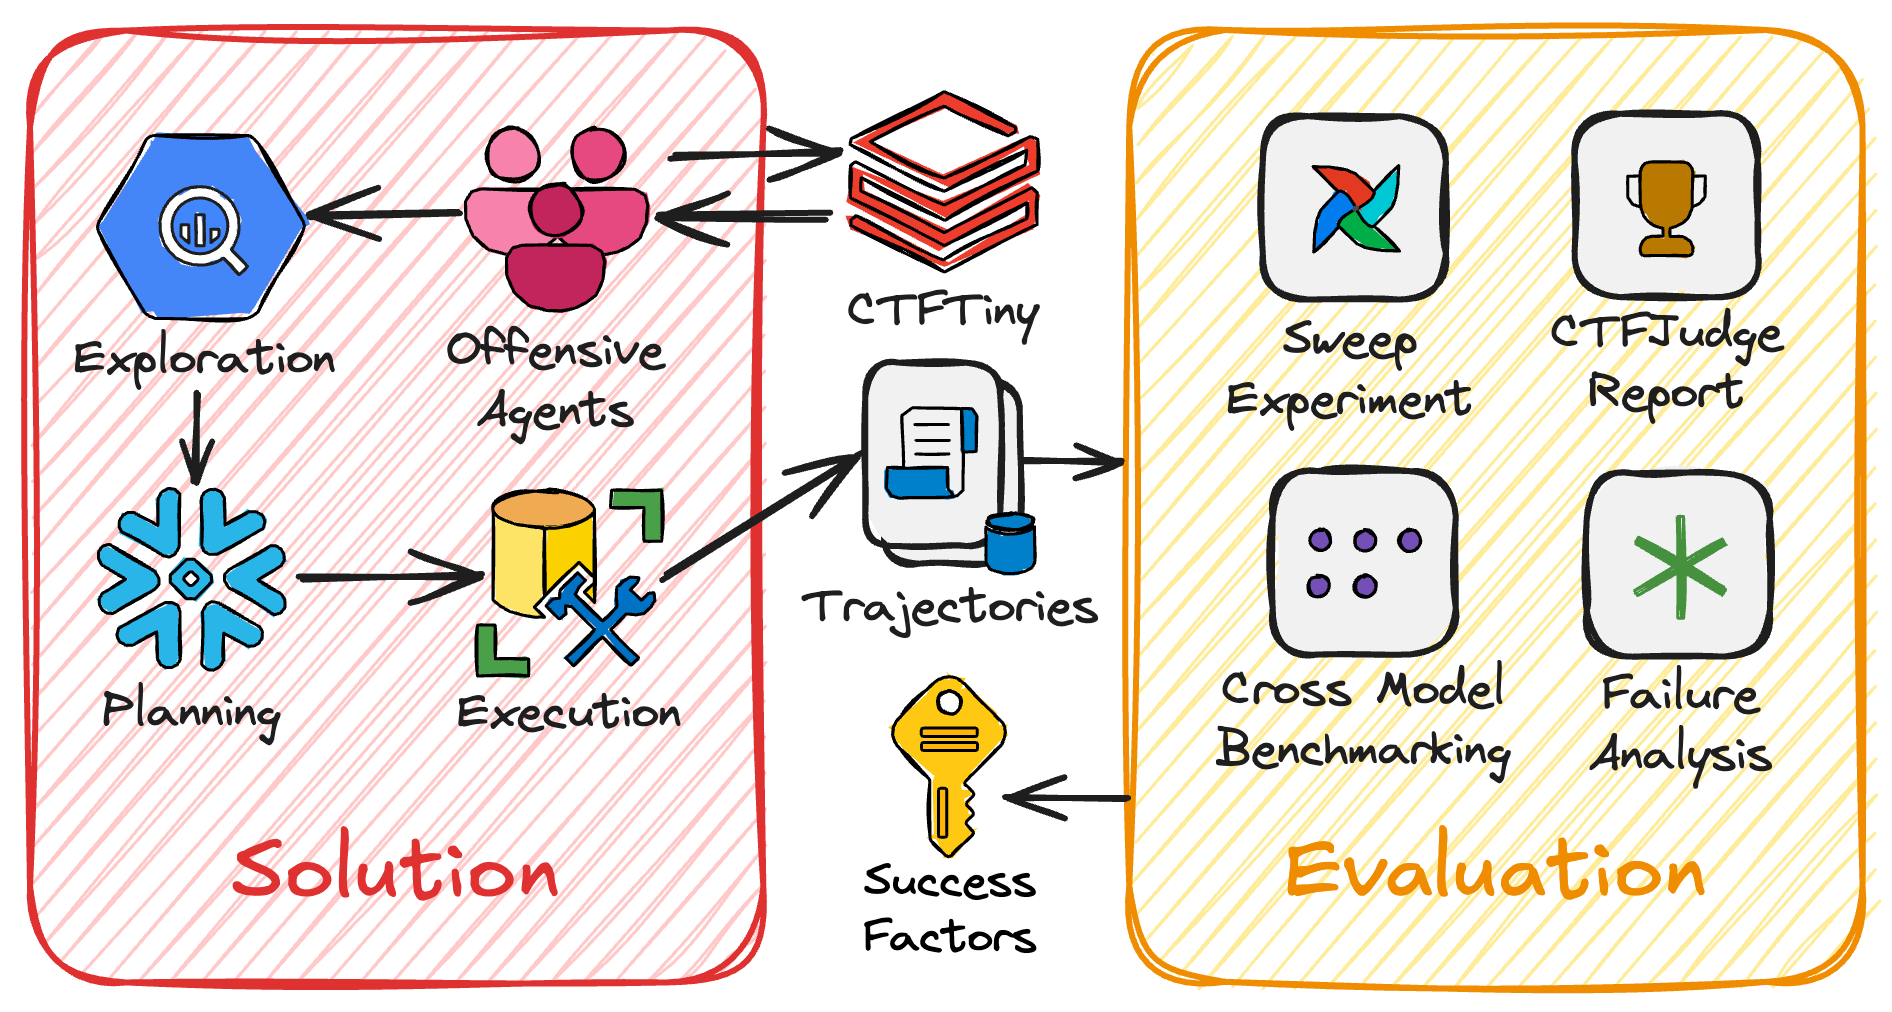
\includegraphics[width=1.1\linewidth]{diagrams/evaluation_framework.png}
\caption{Overview of our evaluation, showing how hyperparameter tuning and multi-agent assessment benchmark LLM-based cybersecurity agents.}
\label{fig:evaluation_farmework}
\end{figure}

CTF challenges require stepwise reasoning, procedural decomposition, command execution, and deep domain knowledge retrieval~\cite{muzsai2024hacksynth,abramovich2024enigma, shao2025craken}. They span various categories, including binary exploitation, reverse engineering, cryptography, web exploitation, and forensics, each demanding different toolchains and strategies. Thus CTFs are ideal for benchmarking offensive security agents to assess reasoning, tool use, and problem solving efficiency.

\texttt{D-CIPHER} is a multi-agent framework where specialized agents coordinate through planning, execution, and feedback to solve CTF problems~\cite{udeshi2025d}. This human-like division of responsibilities improves scalability and modularity in solving diverse challenges. Yet, evaluating agentic systems is an open challenge and many issues need addressing. First, both the agentic system and its LLM operate as black boxes, sensitive to hyperparameter settings such as temperature, top-$p$, iteration limits, and token limits. Prior work did not examine how the hyperparameters affect behavior, performance of the agents and  did not  provide a recipe to study the factors underlying their success.

% Existing research in LLM-agent CTF solving tends to rely on rigid pipelines with fixed prompting strategies or hard-coded plans~\cite{fang2024llm,yang2023language,yao2022react}. While recent works have applied LLM-powered agents to CTF tasks, many rely on static prompting strategies or pre-defined execution flows~\cite{yang2023language,fang2024llm,muzsai2024hacksynth}. Although these methods demonstrate the feasibility of agentic CTF solving, there remains limited understanding of how system-level factors, such as hyperparameters, impact performance across varied challenge types.

In addition to architectural and tuning limitations, evaluation methodologies are in their infancy. Prior work adopts a pass/fail  metric based on whether the agent correctly extracts the flag or whether the agent  completed the human-defined subtasks. This coarse metric doesnt capture nuances such as partial progress, vulnerability detection ability, tool invocation efficiency, and reasoning steps attempted by the agent. This limits our understanding of agentic systems’ cybersecurity capabilities.
Another bottleneck is the lack of standardized, lightweight benchmarks for reproducible experiments. Most CTF datasets are either heavy weight ~\cite{shao2024nyu,zhang2024cybenchframeworkevaluatingcybersecurity,bhatt2024cyberseceval}, or lack systematic difficulty analysis \cite{yang2023intercode}. They are ill-suited for rapid, resource-constrained testing. %This poses challenges for comparing different agentic methods or conducting controlled parameter studies.

To address these limitations, we present a comprehensive study on offensive security agents. Our work includes an LLM judge agent for fine-grained assessment of the offensive reasoning capabilities of such systems, in-depth evaluation of key hyperparameters, and the use of a lightweight benchmark. Figure~\ref{fig:evaluation_farmework} illustrates the overall workflow of our evaluation pipeline, which integrates hyperparameter tuning, multi-agent coordination, and multi-dimensional evaluation on a standardized benchmark.
By bridging methodological rigor with practical benchmarking, our framework not only supports the design of effective offensive security agents, but also offers a foundation for assessing agentic reasoning. %We hope this work inspires future research into adaptive agents, explainable tool use, and performance-aware coordination in high-stakes domains like CTFs.
Our contributions are threefold:
\begin{itemize}
\item Empirical analysis of offensive security agent system to show how hyperparameters (e.g., temperature, top-$p$, and max tokens) affect performance, offering insights.
\item \texttt{CTFJudge}, a fine-grained framework that assesses offensive security agents across aspects like vulnerability reasoning and exploitation techniques, uncovering bottlenecks beyond pass/fail metrics.
\item \texttt{CTFTiny} is a curated set of 50 real-world CTF tasks spanning six domains, enabling reproducible, low-cost evaluation and parameter studies.
\end{itemize}


% %Judge-based agent and propose the new metrics rather than binary
% %Comprehensive evaluation
% %CTFTiny benchmark
% The growing capabilities of large language models (LLMs) have enabled a new class of agentic systems capable of performing complex reasoning tasks in domains such as cybersecurity. These systems can be configured as autonomous agents that plan, reason, and interact with tools to solve problems traditionally requiring expert human intervention~\cite{wang2024surveyllmagents,guo2024largelanguagemodelbased,motlagh2024large}. In recent years, this paradigm has shown significant promise in the context of Capture the Flag (CTF) challenges, which represent practical, scenario-driven exercises used to evaluate offensive security skills~\cite{yang2023language,shao2024empirical,tann2023using}.

% \begin{figure}[t!]
%     \centering
%     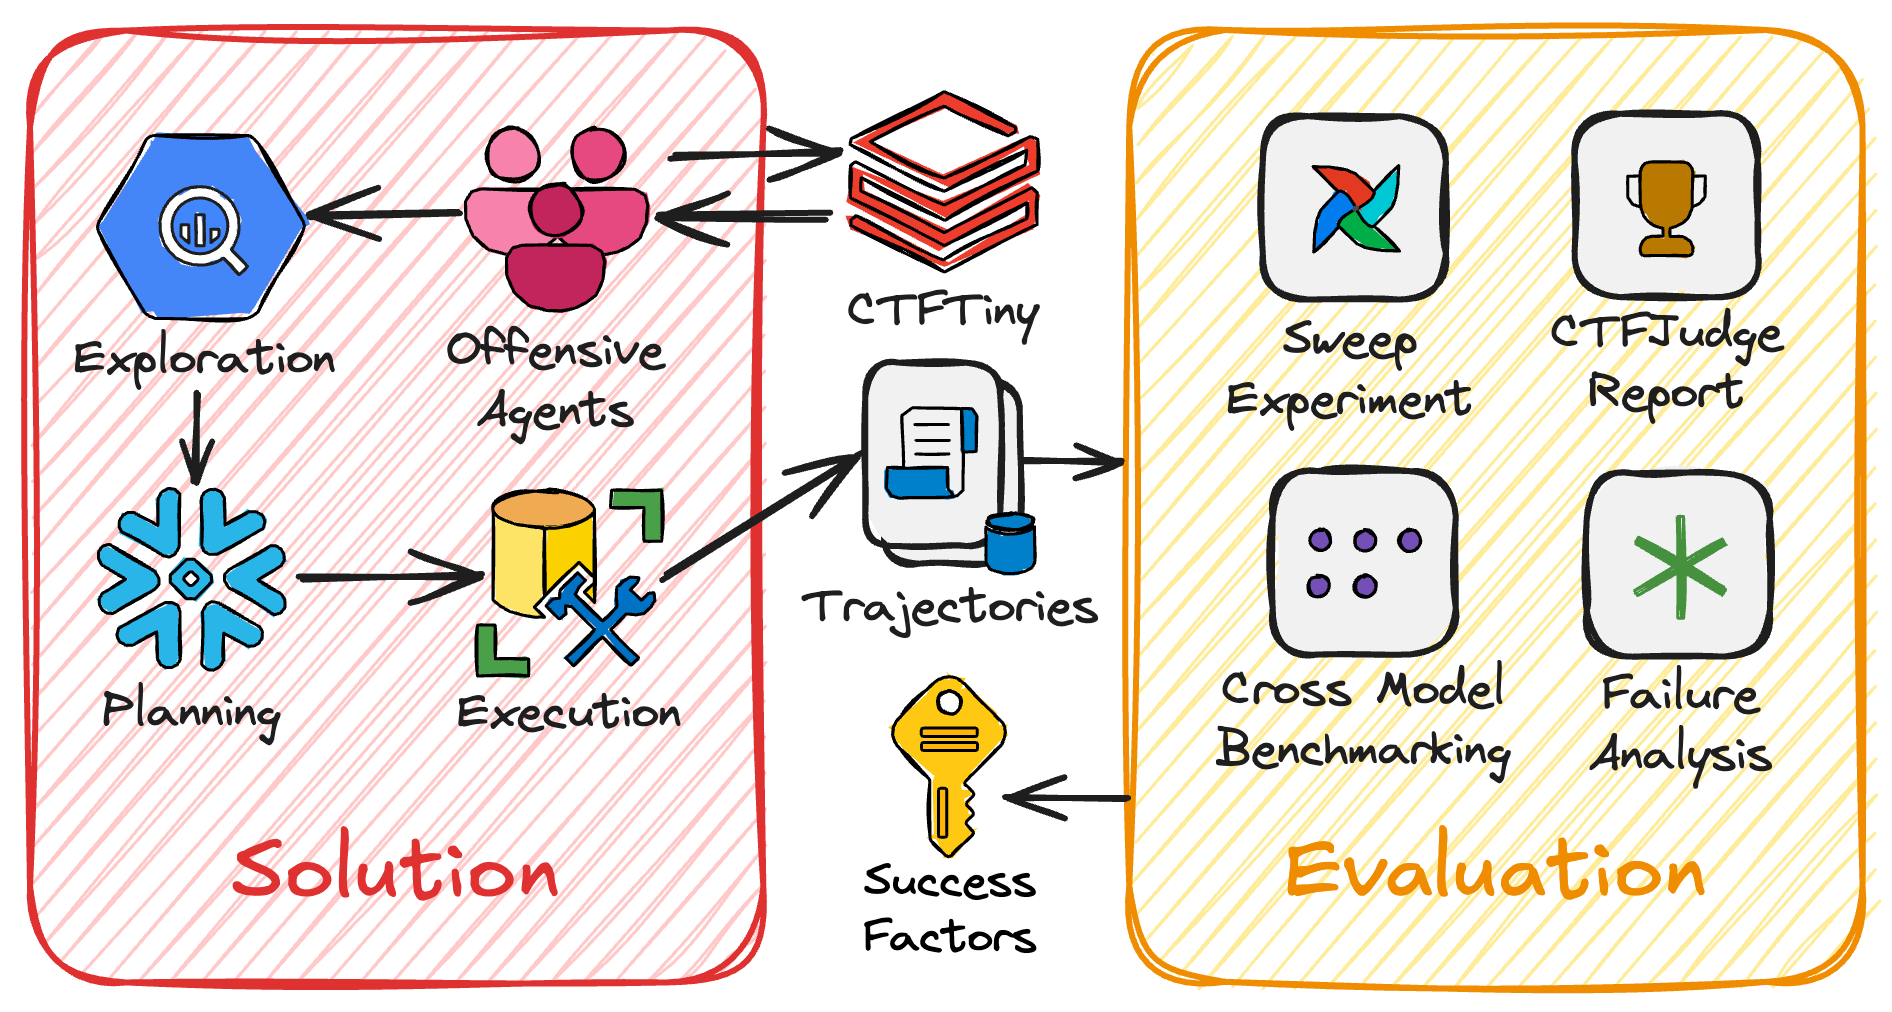
\includegraphics[width=\linewidth]{diagrams/evaluation_framework.png}
%     \caption{Overall workflow of our evaluation.}
%     \label{fig:evaluation_farmework}
% \end{figure}

% Solving CTF challenges is inherently complex, often requiring multi-step reasoning, procedural decomposition, external tool invocation, and domain-specific knowledge retrieval~\cite{yang2023language,muzsai2024hacksynth,abramovich2024enigma}. Challenges span diverse categories such as binary exploitation, reverse engineering, cryptography, web exploitation, and forensics, each demanding distinct technical strategies. The diversity and depth of these challenges make them an ideal testbed for evaluating the reasoning and tool-using capabilities of agentic LLM-based systems.

% To effectively address the demands of such scenarios, one of the recent work presented a collaborative multi-agent architecture, \texttt{D-CIPHER}, in which specialized agents coordinate to analyze, decompose, and solve CTF tasks~\cite{udeshi2025d}. This division of responsibility across planning, execution, and feedback mechanisms mirrors human teamwork and enables scalable problem-solving. However, the performance of such multi-agent systems is highly sensitive to their underlying hyperparameters, such as temperature, top-p, and max token. This necessitates a rigorous and systematic exploration of these parameters to fully realize the potential of agentic systems in automated cybersecurity reasoning.

% While recent efforts have explored the application of LLM-powered agents to solve CTF challenges, most of these systems follow static, pre-defined pipelines without adapting their internal strategies based on task complexity or challenge type~\cite{yang2023language,fang2024llm,muzsai2024hacksynth}. These approaches often hard-code planning logic or rely on fixed prompting templates, limiting their flexibility and effectiveness across diverse problem categories~\cite{yao2022react,shin-etal-2020-autoprompt}.

% Moreover, despite the growing use of agentic architectures, there has been limited focus on understanding how different hyperparameters affect overall system performance. Critical parameters such as temperature, top-p sampling, and max token are typically tuned heuristically or left at default values, with minimal analysis of their broader impact~\cite{yang2023intercode,zhang2023automatic}. This lack of systematic hyperparameter evaluation hinders progress toward more robust and generalizable agent designs.

% In addition, the research community currently lacks lightweight, standardized datasets that enable consistent and reproducible evaluation of agentic systems in the CTF domain. Existing CTF benchmarks are often large, fragmented, or tailored for human solvers, making them less suitable for constrained experiments or ablation studies because of high cost~\cite{shao2024nyu,zhang2024cybenchframeworkevaluatingcybersecurity,bhatt2024cyberseceval}. As a result, comparing different agentic methods or evaluating incremental improvements remains a challenge. This underscores the need for a compact yet representative dataset that supports controlled experimentation and rapid iteration.

% Further, the evaluation of such agentic systems are limited to whether agents are able to figure out flag or not (kind of binary decision). The capability of agentic systems to understand the environment, vulnerability detection, exploitation efficency etc. Therefore, there is a need for framework to asssess these performance metric to provide more granual capability of these agentic system for offensive reasoning.

% To address the limitations outlined above, we present a systematic study that advances both the design and evaluation of agentic systems for automated CTF solving. The overall worklflow of our evaluation is shown in Fig~\ref{fig:evaluation_farmework}. Building on our multi-agent framework \texttt{D-CIPHER}, we make the following key contributions:
% \begin{itemize}
%     \item \textbf{Hyperparameter-Centric Analysis:} We perform an extensive evaluation of \texttt{D-CIPHER} by varying core hyperparameters such as temperature, top-p sampling, iteration limits, and agent coordination strategies. Our experiments reveal how these parameters influence performance across different CTF categories, offering practical guidance for tuning agentic systems.
%     \item \textbf{CTFTiny Benchmark Dataset:} We introduce \texttt{CTFTiny}, a curated set of $50$ real-world CTF challenges spanning five major categories. Designed for lightweight yet meaningful evaluation, this dataset enables reproducible, controlled experiments in computationally constrained environments.
%     \item \textbf{Foundation for Future Research:} By combining systematic experimentation with the release of a standard benchmark, this work establishes a reusable foundation for advancing agentic reasoning in cybersecurity. \texttt{CTFTiny} fills a critical gap in the ecosystem by supporting fair comparisons and facilitating iterative development of language-agent systems.
% \end{itemize}

% \charan{Contribution 2 and 3 looks similar; No Discussion about exploration vs exploitation; why ? }
% \minghao{Since we removed the action analysis part, we can revise the introduction section}
% \nanda{Update citation and proofread}
